\documentclass[a4paper]{article} %doctype define
\usepackage[a4paper,hmargin={3cm,2.5cm},vmargin={2.5cm,2.5cm}]{geometry} %setup margins
\usepackage[utf8]{inputenc} %for special character support
\usepackage{graphicx}   %for defining images root folder below
\graphicspath{ {images/} }
\usepackage{hyperref} %link table of content with actual text part

%===============For Code visibility======================
\usepackage{listings}

\usepackage{xcolor} %define custom colors
\definecolor{mygreen}{rgb}{0,0.6,0}
\definecolor{mygray}{rgb}{0.5,0.5,0.5}
\definecolor{mymauve}{rgb}{0.58,0,0.82}
\definecolor{compilerRed}{HTML}{cc0000}

\lstset{
    backgroundcolor=\color{white},      % choose the background color; you must add \usepackage{color} or \usepackage{xcolor}; should come as last argument
    language=[x86masm]Assembler,                    % the language of the code
    basicstyle=\footnotesize\ttfamily,  % the size of the fonts that are used for the code
    % breakatwhitespace=false,            % sets if automatic breaks should only happen at whitespace
    % breaklines=true,                    % sets automatic line breaking
    captionpos=b,                       % sets the caption-position to bottom
    commentstyle=\color{mygreen},       % comment style
    % deletekeywords={...},               % if you want to delete keywords from the given language
    % escapeinside={\%*}{*)},             % if you want to add LaTeX within your code
    % extendedchars=true,                 % lets you use non-ASCII characters; for 8-bits encodings only, does not work with UTF-8
    firstnumber=1,                      % start line enumeration with line 1
    numbers=left,                       % where to put the line-numbers; possible values are (none, left, right)
    numberstyle=\tiny\color{mygray},    % the style that is used for the line-numbers
    numbersep=7pt,                      % how far the line-numbers are from the code
	frame=single,                       % code snippet frame, t-> top, b->bottom, l->left, r->right, single-> all around
	tabsize=4,                          % tab = (tabsize) * space
    columns=flexible,                   % two options, fixed or flexible
    keepspaces=true,                    % keeps spaces in text, useful for keeping indentation of code (possibly needs columns=flexible)
    morekeywords={*,MVI,DAD,INX,DCR,LXI,DCX,ORA,LDAX,ANI,INR,LHLD,RAL,SIM,RIM,XTHL,CPI,RAR,RNC,EI,...},               % if you want to add more keywords to the set
    rulecolor=\color{black},            % if not set, the frame-color may be changed on line-breaks within not-black text (e.g. comments (green here))
	showspaces=false,                   % show spaces everywhere adding particular underscores; it overrides 'showstringspaces'
    showstringspaces=false,             % underline spaces within strings only
    showtabs=false,                     % show tabs within strings adding particular underscores
    stepnumber=1,                       % the step between two line-numbers. If it's 1, each line will be numbered
    stringstyle=\color{mymauve},        % string literal style
    title=\small\lstname,               % show the filename of files included with \lstinputlisting; also try caption instead of title
	% keepspaces,
	keywordstyle=\color{blue},           % keyword style    
    morecomment=[l][\color{compilerRed}]{\#}
}
%========================== For images=================
\usepackage{caption}
\usepackage{subcaption}

%==================== START================
\begin{document}


\begin{titlepage}
    \begin{center}
        \vspace*{1cm}
 
        \huge
            \textbf{Microprocessor Lab Report}\\
        \vspace{1cm}
        \large
            \textbf{Abhiroop Mukherjee}\\
            \textbf{Enrl. No: 510519109}\\
        \vspace{1cm}
        
\includegraphics[width=0.4\textwidth]{IIESTS-Logo.png}\\
        \vspace{1cm}
        \normalsize
        Department of Computer Science and Technology\\
        Indian Institute of Engineering Science and Technology, Shibpur 
 
        \vfill               
    \end{center}
 \end{titlepage} %Title Page

\pagenumbering{roman}
\setcounter{tocdepth}{1} % only allow 1 nests
\tableofcontents
\newpage
\pagenumbering{arabic}
\setcounter{page}{1}
% ==================MAIN TEXT========================
\section[Find out the sum of the first 30 natural numbers]{Assignment 1} %[toc content]{text content}
    \subsection{Objective}
        Find out the sum of the first 30 natural numbers.
    \subsection{Tool/Experimental setup considered}
        \begin{itemize}
            \item Jubin's 8085 Simulator
        \end{itemize}
    \subsection{Procedure}
        We know that
        \[1 + 2 + 3 + ... + 29 + 30 = \frac{30 \times 29}{2} = 435 =  01D1H\]
        This result is not possible to store in a single register, so we need to use register pair to store the result.
    \subsection{Program}
        \lstinputlisting[caption=assembly program to find sum of the first 30 natural numbers]{./../Programs/Assignment 1/1_1_sum till 30.asm}
    \subsection{Experimentation}
        \begin{figure}[h!]
            \centering
            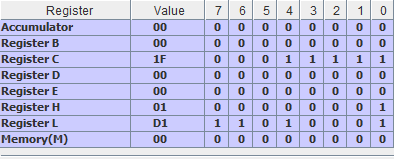
\includegraphics[width=0.7\textwidth]{Assignment 1/1_sum_till_30/registor.png}
            \caption{Register configuration after execution (observe HL)}
            \label{fg1}
        \end{figure}
    \subsection{Conclusion}
        We see that after the execution of program, the data stored in HL register pair is 01D1H, which is the hexadecimal value of 435.\\
        Hence the program is working as expected.
\newpage

\section[Find minimum and maximum number in 10-byte unsigned array]{Assignment 2} %[toc content]{text content}
    \subsection{Objective}
        From an array of 10-byte size integers (unsigned) find out the maximum and minimum.
    \subsection{Tool/Experimental setup considered}
        \begin{itemize}
            \item Jubin's 8085 Simulator
        \end{itemize}
    \subsection{Procedure}
        The idea is to linearly iterate through all the values of the arr, and update the register for minimum(C) and maximum(B) values.
    \subsection{Program}
        \lstinputlisting[caption=assembly program to find minimum and maximum number in 10-byte unsigned array]{./../Programs/Assignment 1/1_2_min-max of 10 size array.asm}
    \subsection{Experimentation}
        \begin{figure}[h!]
            \centering
            \begin{subfigure}[b]{0.4\linewidth}
                \centering
                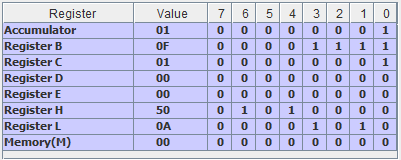
\includegraphics[width=\linewidth]{Assignment 1/2_min-max-10-elem/test 1.png}
                \caption{result for \{5,2,3,4,F,C,7,A,B,1\}}
                \label{fg2a}
            \end{subfigure}
            \begin{subfigure}[b]{0.4\linewidth}
                \centering
                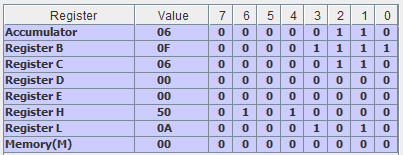
\includegraphics[width=\linewidth]{Assignment 1/2_min-max-10-elem/test 2.png}
                \caption{result for \{F,E,D,C,B,A,9,8,7,6\}}
                \label{fg2b}
            \end{subfigure}
            \caption{Result for different inputs}
            \label{fg2}
        \end{figure}
    \subsection{Conclusion}
        We see that that after program execution, B has the maximum value of array, and C has the minimum value of the array.\\
        Hence the program is working as expected.
\newpage

\section[Delay Procedure]{Assignment 3} %[toc content]{text content}
    \subsection{Objective}
        Write a routine that produces a delay. The delay value must be passed to register pair DE.
    \subsection{Tool/Experimental setup considered}
        \begin{itemize}
            \item Jubin's 8085 Simulator
        \end{itemize}
    \subsection{Procedure}
        Idea is to assign DE a very big value (say FFFF), and decrement it in a loop till DE becomes 0 to produce delay in execution.
    \subsection{Program}
        \lstinputlisting[caption=assembly program to produce delay]{./../Programs/Assignment 1/1_3_delay.asm}
    \subsection{Conclusion}
        We see that the code runs for sometime, then completes it's execution, signifying that the delay function worked and delayed execution of CPU for some time.\\
        Hence the program is working as expected.
\newpage

\section[Move block of data from location X to location Y]{Assignment 4} %[toc content]{text content}
    \subsection{Objective}
        Write a subroutine to move a block of bytes from location X to location Y.\\
        Note that the caller would specify
        \begin{itemize}
            \item X, the source address
            \item Y, the destination address
            \item Z, the block size
        \end{itemize}
        Note that X, Y and Z are 16-bit quantities.
    \subsection{Tool/Experimental setup considered}
        \begin{itemize}
            \item Jubin's 8085 Simulator
        \end{itemize}
    \subsection{Procedure}
        Start reading numbers from location X and save them to location Y, after each iteration, update address of X and Y to next byte. Do this Z times and the whole block is copied.
    \subsection{Program}
        \lstinputlisting[caption=assembly program to move block]{./../Programs/Assignment 2/2_1_move_array.asm}
        \newpage
    \subsection{Experimentation}
        \begin{figure}[h!]
            \centering
            \begin{subfigure}[b]{0.49\linewidth}
                \centering
                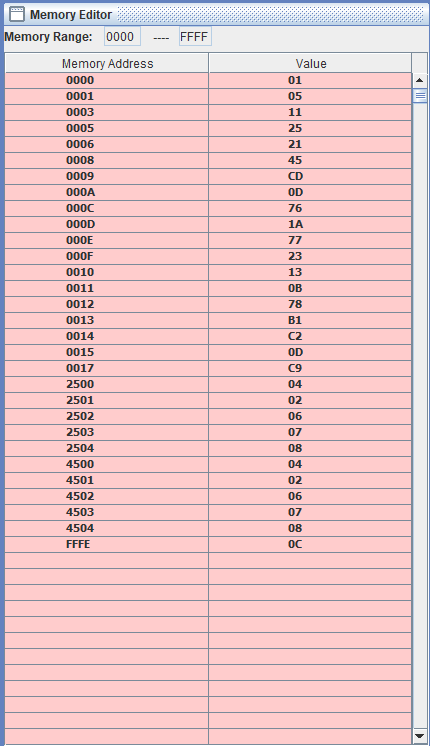
\includegraphics[width=\linewidth]{Assignment 2/1_Move Blocks/5 data copy.png}
                \caption{result for \{4,2,6,7,8\}}
                \label{fg3a}
            \end{subfigure}
            \begin{subfigure}[b]{0.49\linewidth}
                \centering
                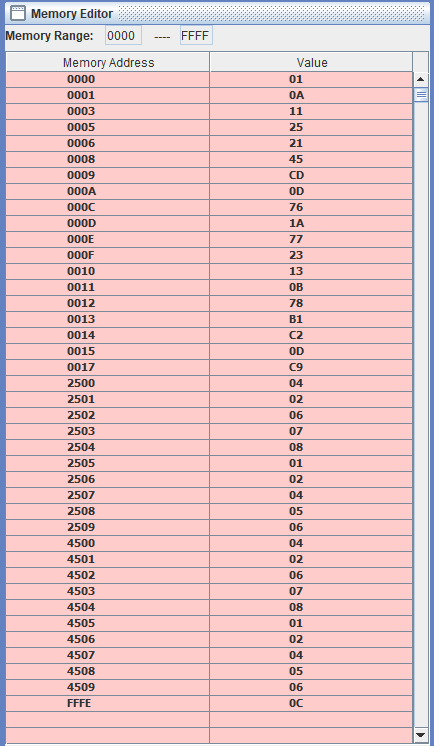
\includegraphics[width=\linewidth]{Assignment 2/1_Move Blocks/10 data copy.png}
                \caption{result for \{4,2,6,7,8,1,2,4,5,6\}}
                \label{fg3b}
            \end{subfigure}
            \caption{Result for different inputs}
            \label{fg3}
        \end{figure}
    \subsection{Conclusion}
        We see that all the data from location 2500(X) to (2500 + Z) has been copied to location 4500(Y) to (4500 + Z) [Z is 5 in \ref{fg3a} and 10 in \ref{fg3b}].\\
        Hence the program is working as expected.
\newpage

\section[Check if number odd]{Assignment 5} %[toc content]{text content}
    \subsection{Objective}
        Write a function isODD(unsigned n) in assembly that takes an unsigned integer (a byte) and determines if it is odd (returns 1) or 0 if it is even.
    \subsection{Tool/Experimental setup considered}
        \begin{itemize}
            \item Jubin's 8085 Simulator
        \end{itemize}
    \subsection{Procedure}
        Odd numbers will always be in the form of $2x + 1$, which means that they will have 1 as their LSB.\\
        So we just check if $number \land 01$ is 1 or not. If the result is 1, then the number is odd, else it is even.
    \subsection{Program}
        \lstinputlisting[caption=assembly program to check if given number isOdd or not]{./../Programs/Assignment 2/2_2_is_Odd.asm}
    \subsection{Experimentation}
        \begin{figure}[h!]
            \centering
            \begin{subfigure}[b]{0.49\linewidth}
                \centering
                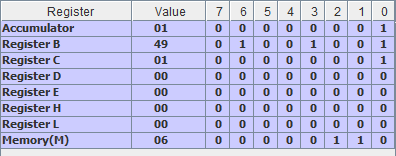
\includegraphics[width=\linewidth]{Assignment 2/2_isodd/odd73.png}
                \caption{result for odd number(73)}
                \label{fg4a}
            \end{subfigure}
            \begin{subfigure}[b]{0.49\linewidth}
                \centering
                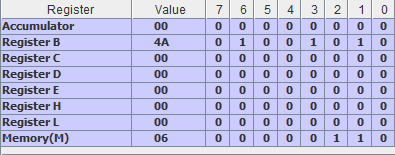
\includegraphics[width=\linewidth]{Assignment 2/2_isodd/even74.png}
                \caption{result for even number(73)}
                \label{fg4b}
            \end{subfigure}
            \caption{Result for both even and odd numbers}
            \label{fg4}
        \end{figure}
    \subsection{Conclusion}
        We see that in case of odd number, C is 1 after execution and in case of even number, C is 0 after execution.\\
        Hence the program is working as expected.
\newpage

\section[Multi-Byte Addition]{Assignment 6} %[toc content]{text content}
    \subsection{Objective}
        Write a function to add two multi-byte numbers stored in location X and Y. The result is stored in X. Pass a parameter Z indicating the no. of bytes to be added.
    \subsection{Tool/Experimental setup considered}
        \begin{itemize}
            \item Jubin's 8085 Simulator
        \end{itemize}
    \subsection{Procedure}
        We simulate the default way of adding numbers, we go from right to left, adding (with carry) the numbers and adding it to stack, then we keep popping the elements and save it in X.
    \subsection{Program}
        \lstinputlisting[caption=assembly program to add multi-byte numbers]{./../Programs/Assignment 2/2_3_byte_add_right_to_left.asm}
        \newpage
    \subsection{Experimentation}
        \begin{figure}[h!]
            \centering
            \begin{subfigure}[b]{0.49\linewidth}
                \centering
                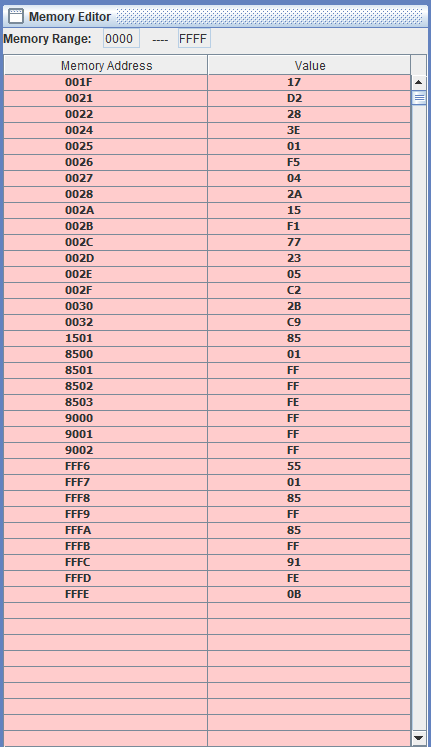
\includegraphics[width=\linewidth]{Assignment 2/3_multibyte_add/FFFFFF_FFFFFF.png}
                \caption{result for \{FF,FF,FF\} + \{FF,FF,FF\}}
                \label{fg5a}
            \end{subfigure}
            \begin{subfigure}[b]{0.49\linewidth}
                \centering
                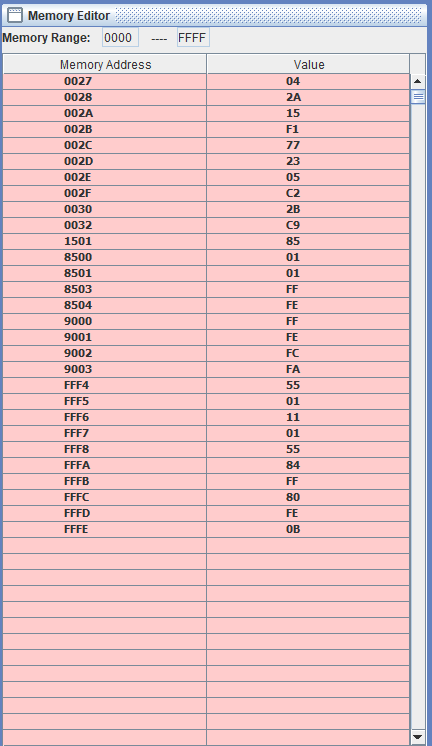
\includegraphics[width=\linewidth]{Assignment 2/3_multibyte_add/01020304_FFFEFCFA.png}
                \caption{result for \{01,02,03,04\} + \{FF,FE,FC,FA\}}
                \label{fg5b}
            \end{subfigure}
            \caption{Result of multi-byte addition (start looking from address 8500)}
            \label{fg5}
        \end{figure}
    \subsection{Conclusion}
        We see that the result of multi-byte addition is correct.\\
        Hence the program is working as expected.
\newpage

\section[Fast Multiplication Subroutine]{Assignment 7} %[toc content]{text content}
    \subsection{Objective}
        Write a fast sub-routine to multiply 9 by 15.
    \subsection{Tool/Experimental setup considered}
        \begin{itemize}
            \item Jubin's 8085 Simulator
        \end{itemize}
    \subsection{Procedure}
        We use the Shift-and-Add Multiplication to fast multiply 15 and 9, as register size is 8 bits, we can do this multiplication by using a loop which runs 8 times, i.e O(1)\\
        This method is faster than default loop method, which run in O(min(m, n)), where m and n are the numbers that will be multiplied.
    \subsection{Program}
        \lstinputlisting[caption=assembly program to fast multiply 15 times 9]{./../Programs/Assignment 3/3_1_9_times_15_shift.asm}
    \subsection{Experimentation}
        \begin{figure}[h!]
            \centering
            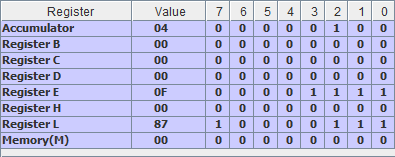
\includegraphics[width=0.7\textwidth]{Assignment 3/1_9x15/9x15.png}
            \caption{Register configuration after execution (look at HL)}
            \label{fg6}
        \end{figure}
    \subsection{Conclusion}
        $9\times15=135 = 0087H$\\
        We see that the result in HL register is same as what we expected.\\
        Hence the program is working as expected.
\newpage

\section[Sort Subroutine]{Assignment 8} %[toc content]{text content}
    \subsection{Objective}
        Write a subroutine to sort a 5-element byte array (Any algorithm will do)
    \subsection{Tool/Experimental setup considered}
        \begin{itemize}
            \item Jubin's 8085 Simulator
        \end{itemize}
    \subsection{Procedure}
        We use bubble sort algorithm to sort the array.
    \subsection{Program}
        \lstinputlisting[caption=assembly program to bubble sort array]{./../Programs/Assignment 3/3_2_bubble_sort_5_elem.asm}
        \newpage
    \subsection{Experimentation}
        \begin{figure}[h!]
            \centering
            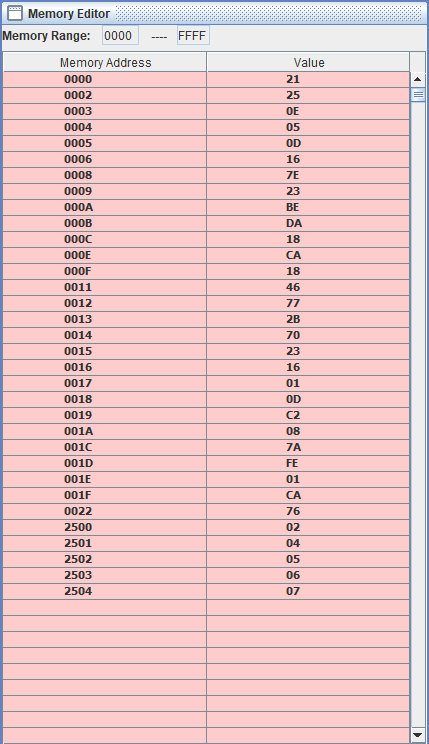
\includegraphics[width=0.7\textwidth]{Assignment 3/2_sort/mem_output.png}
            \caption{Register configuration after execution (look from address 2500)}
            \label{fg7}
        \end{figure}
    \subsection{Conclusion}
        We see that after program execution, values of address 2500 - 2504 is sorted in ascending order.\\
        Hence the program is working as expected.
\newpage

\section[Subroutine to save Register Status]{Assignment 9} %[toc content]{text content}
    \subsection{Objective}
        Write a sub-routine to store all the registers (A, F, B, C, D, E, H, L, I, SPL, SPH, PCL, PC, in that order) starting from location MYREGISTERS.
    \subsection{Tool/Experimental setup considered}
        \begin{itemize}
            \item Jubin's 8085 Simulator
        \end{itemize}
    \subsection{Program}
        \lstinputlisting[caption=assembly program to store register configuration]{./../Programs/Assignment 3/3_3_store_all_reg.asm}
        \newpage
    \subsection{Experimentation}
        \begin{figure}[h!]
            \centering
            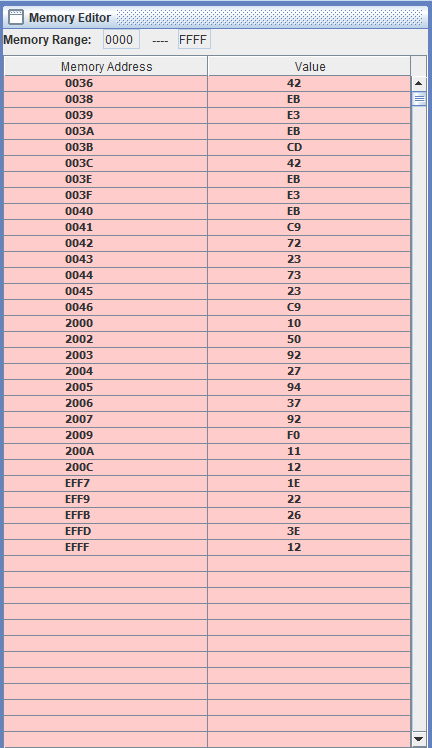
\includegraphics[width=0.7\textwidth]{Assignment 3/3_save_reg_config/mem.png}
            \caption{Register configuration after execution (look from address 2000)}
            \label{fg8}
        \end{figure}
    \subsection{Conclusion}
        We see that after program execution, all the predefined value of registers are stored in memory starting from address 2000.\\
        Hence the program is working as expected.
\newpage

\section[POST to check stuck at 1 fault]{Assignment 10} %[toc content]{text content}
    \subsection{Objective}
        Implement a POST or power-on-self-test  where each RAM location is tested for stuck-at-zero or stuck-at-one fault. 
        In your case the function takes the start address of the RAM block and the block size in bytes.
        The function sets CY in case of any error (else it is set to 0); HL contains the faulty location and Acc contains 0 for stuck at zero fault and 1 for stuck at one fault.
        [Note: usually there wont be any error as your RAM is not faulty, so direct checking may not set CY flag]
    \subsection{Tool/Experimental setup considered}
        \begin{itemize}
            \item Jubin's 8085 Simulator
        \end{itemize}
    \subsection{Procedure}
        We iteratively go through STARTLOC to (STARTLOC + LEN) and check if any value is 1 or not, if it is, we exit from there setting the C flag.
    \subsection{Program}
        \lstinputlisting[caption=assembly program for POST for stuck at 1 fault]{./../Programs/Assignment 4/4_1_POST.asm}
        \newpage
    \subsection{Experimentation}
    \begin{figure}[h!]
        \centering
        \begin{subfigure}[b]{0.49\linewidth}
            \centering
            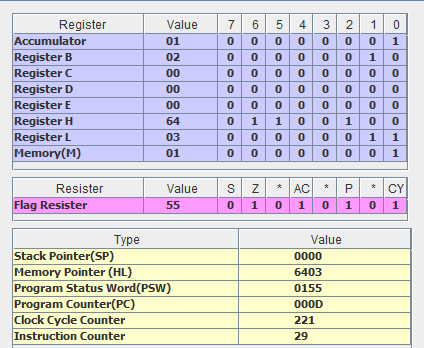
\includegraphics[width=\linewidth]{Assignment 4/1_POST/yes_stuck.png}
            \caption{result of the program}
            \label{fg9a}
        \end{subfigure}
        \begin{subfigure}[b]{0.49\linewidth}
            \centering
            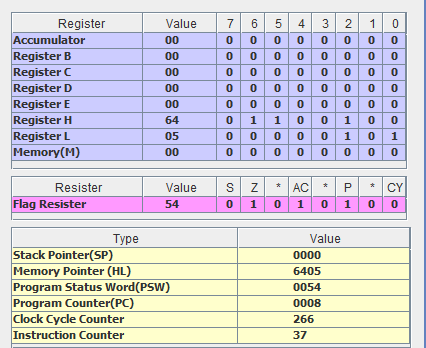
\includegraphics[width=\linewidth]{Assignment 4/1_POST/no_stuck.png}
            \caption{result of the program if we comment line 4 and 5}
            \label{fg9b}
        \end{subfigure}
        \caption{Result of Program Execution}
        \label{fg9}
    \end{figure}
    \subsection{Conclusion}
        We see that if there exist a 1 in some memory location, the program sets Cy flag and HL register to stuck address; when there is no 1 in whole array, C is unset\\
        Hence the program is working as expected.
\newpage

\section[Binary Search]{Assignment 11} %[toc content]{text content}
    \subsection{Objective}
        Implement a binary search ---- the function would take the start address and no. of elements in the array. If successful the function resets CY flag and the HL pair points to the element found else CY is set and the value in HL pair is irrelevant. 
    \subsection{Tool/Experimental setup considered}
        \begin{itemize}
            \item Jubin's 8085 Simulator
        \end{itemize}
    \subsection{Program}
        \lstinputlisting[caption=assembly program for the implementation of Binary Search]{./../Programs/Assignment 4/4_2_Binary_Search.asm}
        \newpage
    \subsection{Experimentation}
    \begin{figure}[h!]
        \centering
        \begin{subfigure}[b]{0.49\linewidth}
            \centering
            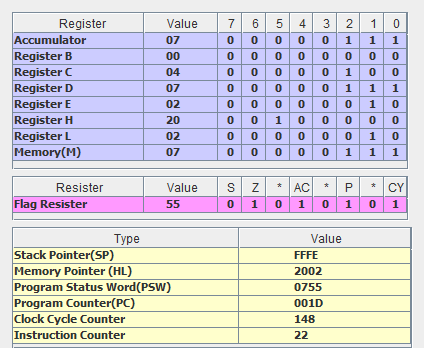
\includegraphics[width=\linewidth]{Assignment 4/2_BS/found.png}
            \caption{result of the program when X is in array}
            \label{fg10a}
        \end{subfigure}
        \begin{subfigure}[b]{0.49\linewidth}
            \centering
            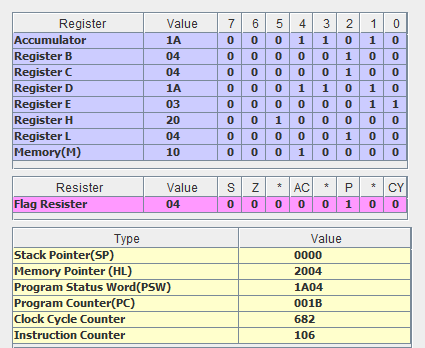
\includegraphics[width=\linewidth]{Assignment 4/2_BS/not_found.png}
            \caption{result of the program when X is not in array}
            \label{fg10b}
        \end{subfigure}
        \caption{Result of Program Execution}
        \label{fg10}
    \end{figure}
    \subsection{Conclusion}
        We see that when X is in array, Cy flag is set and HL points to the data's address in array; but then X is not present, Cy flag is not set.\\
        Hence the program is working as expected.
\newpage

\section[Time Period of a rectangular waveform signal]{Assignment 12} %[toc content]{text content}
    \subsection{Objective}
    Suppose that you are reading a bit of an input port (say, PORT 0) to which the output of a function generator, producing a rectangular wave, is connected. Measure the ON  of this repetitive rectangular waveform time in terms of millisecond.
    \subsection{Procedure}
        \begin{enumerate}
            \item We first wait in an infinite loop, waiting for the signal to turn 0 (in case we started program when signal was already 1).
            \item Then when the signal turns 0, the actual count procedure starts, we again keep waiting in an infinite loop, waiting for the signal to go 1 again.
            \item When the signal goes 1 now, we start counting the amount of time the signal is 1 in another infinite loop.
                \begin{itemize}
                    \item The two register pair is too small to count the number of machine cycles it took for the signal to go to 0.
                    \item so we added a delay (1 ms) after every count, now the count signifies the amount of (1ms) delays it took for signal to go to 0.
                \end{itemize}
            \item now the signal is back to 0, and we have the amount of delays it took for signal to go to 0, we write that data to SAVELOC.
        \end{enumerate}
    \subsection{Program}
        \lstinputlisting[caption=assembly program to calculate time period of rectangular wave]{./../Programs/Assignment 4/4_3_Port.asm}
    \subsection{Conclusion}
        We created a program which will calculate the time period of a rectangular wave as follows
        \[T= BC*(30*1/3 + 1ms) = BC*11ms \pm 2 ms\]
\newpage

\section[Interrupt Service Routine]{Assignment 13} %[toc content]{text content}
    \subsection{Objective}
        \begin{itemize}
            \item Using auto vectored input RST 7.5 prepare a scheme to count the number of key-press done at this interrupting input.
            \item The main routine after initialization of the interrupt mechanism waits in an infinite loop waiting for the key-press. 
            \item On a key-press (that simulates as if you have excited the RST 7.5 input) it increases a counter at a predefined memory location (used to hold the count value).
        \end{itemize}
    \subsection{Tool/Experimental setup considered}
        \begin{itemize}
            \item Jubin's 8085 Simulator
        \end{itemize}
    \subsection{Procedure}
        \begin{enumerate}
            \item We use an RST 7.5 interrupt line to call a procedure every time we get an interrupt.
            \item The Problem is that the computer is so fast that it can take in multiple interrupt in a single button press(click).
            \item To solve this, we disable the interrupt mechanism inside the Interrupt Service Routine, and also add a small delay to make the computer "wait" for the key-press to end.
        \end{enumerate}
    \subsection{Program}
        \lstinputlisting[caption=assembly program to find the number of key presses during the program execution]{./../Programs/Assignment 5/5_1_ISR.asm}
        \newpage
    \subsection{Experimentation}
        \begin{figure}[h!]
            \centering
            \begin{subfigure}[b]{0.49\linewidth}
                \centering
                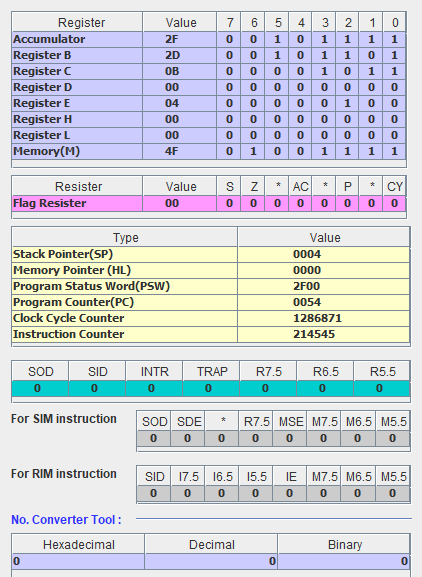
\includegraphics[width=\linewidth]{Assignment 5/1_ISR/4-click.png}
                \caption{register config for 4 interrupt clicks}
                \label{fg11a}
            \end{subfigure}
            \begin{subfigure}[b]{0.49\linewidth}
                \centering
                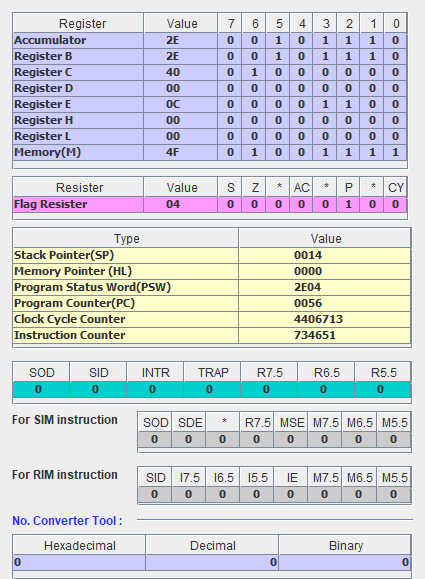
\includegraphics[width=\linewidth]{Assignment 5/1_ISR/12-click.png}
                \caption{register config for 12 interrupt clicks}
                \label{fg11b}
            \end{subfigure}
            \caption{Result of Program Execution (look at DE register pair)}
            \label{fg11}
        \end{figure}
    \subsection{Conclusion}
        We see that the value in DE register pair after program stop matches with the number of clicks made for interrupts.\\
        Hence the program is working as expected.
\newpage

\section[Hardware Debouncing]{Assignment 14} %[toc content]{text content}
    \subsection{Objective}
        Draw the hardware for implementing RST 7.5 based key-press counting -- don't forget to implement h/w based key debouncing problem.
    \subsection{Procedure}
        We previously used software method (using delay) to mitigate debouncing, now we will look into the method to reducing debouncing hardware wise.\par
        One of the simplest hardware-based switch debounce solutions employs a resistor-capacitor (RC) network in conjunction with a switch (i.e our key).

        \begin{figure}[h!]
            \centering
            \fbox{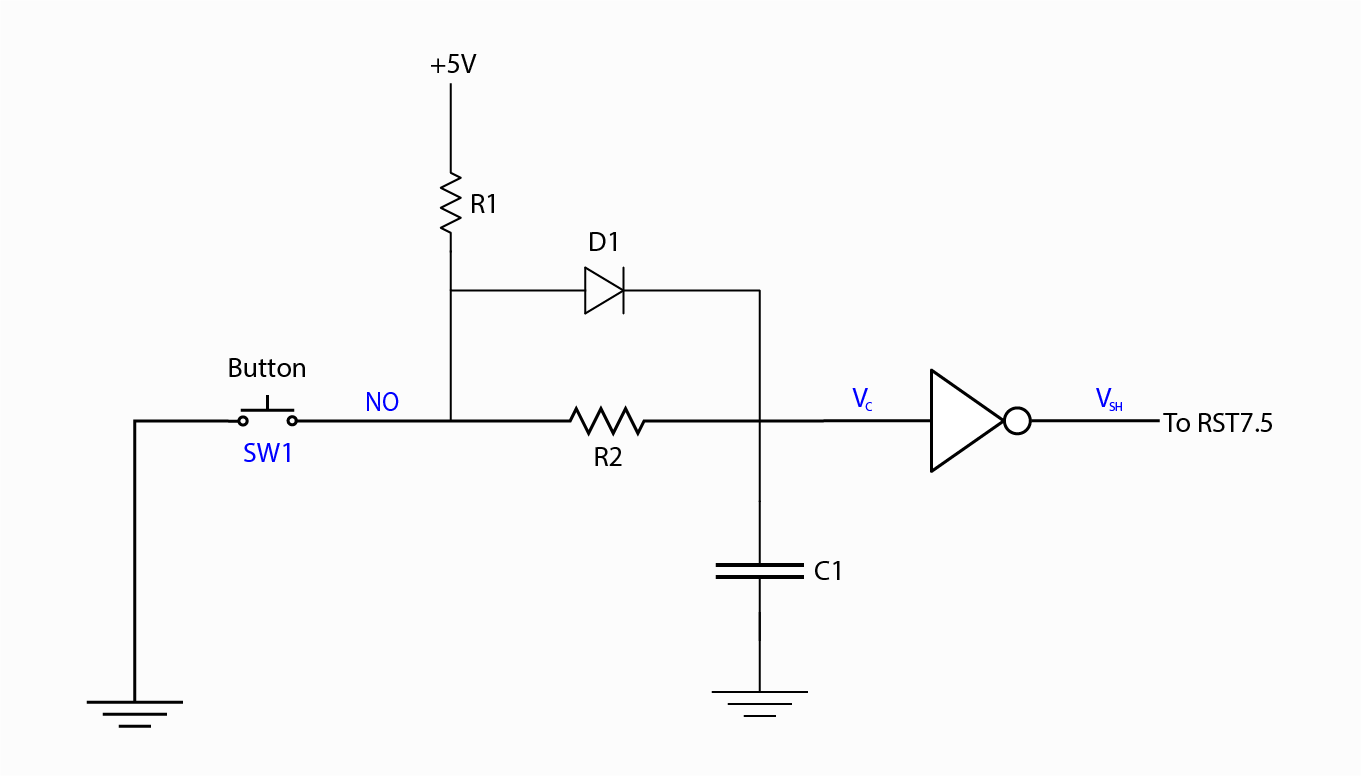
\includegraphics[width=0.8\textwidth]{Assignment 5/2_hardware debouncing/default circuit.png}}
            \caption{Hardware based Switch Debouncing}
            \label{fg12}
        \end{figure}

        When the key is not pressed, there is a way for the power to go from +ve to ground via R1, D1 and C1, which keeps $V_c$ as high, and $V_{sh}$ as low as shown in \ref{fg13a}.\par
        When the key is pressed, the circuit is shorted due to the new circuit and $V_c$ becomes low, making $V_{sh}$ as high as shown in \ref{fg13b}\par
        The capacitor is used to remove the false signals due to debouncing and providing a smoother gradient towards On and Off as shown in \ref{fg14}

        \begin{figure}[h!]
            \centering
            \begin{subfigure}[b]{0.49\linewidth}
                \centering
                \fbox{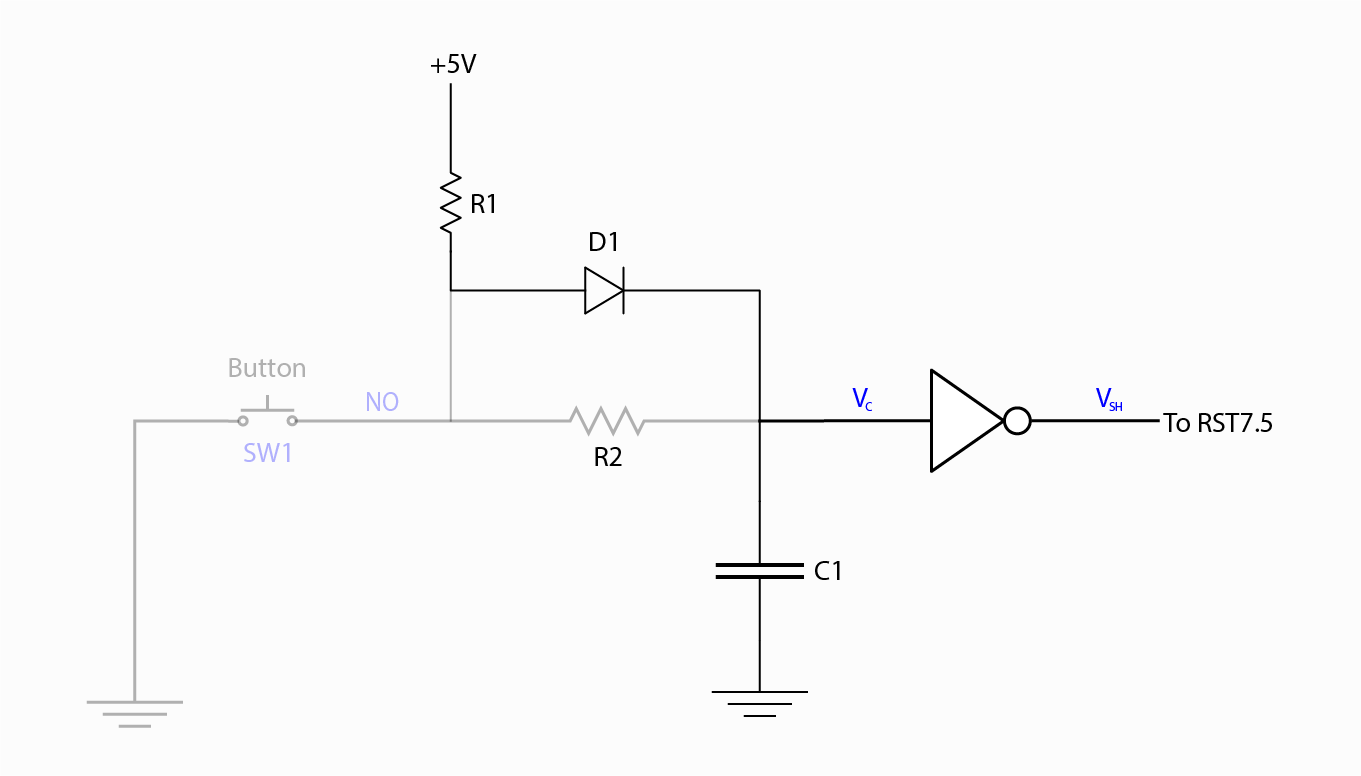
\includegraphics[width=0.95\linewidth]{Assignment 5/2_hardware debouncing/not pressed.png}}
                \caption{Circuit when key is not pressed}
                \label{fg13a}
            \end{subfigure}
            \begin{subfigure}[b]{0.49\linewidth}
                \centering
                \fbox{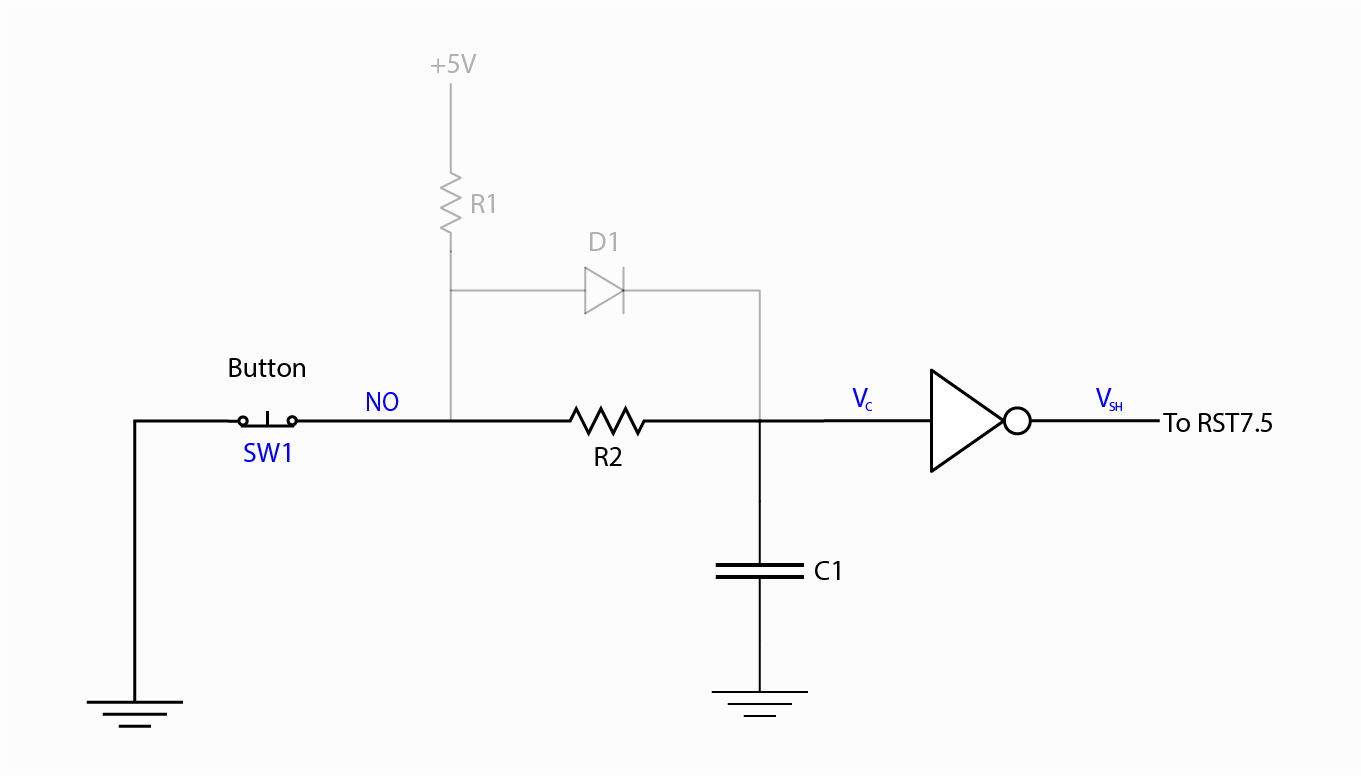
\includegraphics[width=0.95\linewidth]{Assignment 5/2_hardware debouncing/pressed.png}}
                \caption{Circuit when key is pressed}
                \label{fg13b}
            \end{subfigure}
            \caption{Hardware based Switch Debouncing}
            \label{fg13}
        \end{figure}
    \newpage
        
        \begin{figure}[h!]
            \centering
            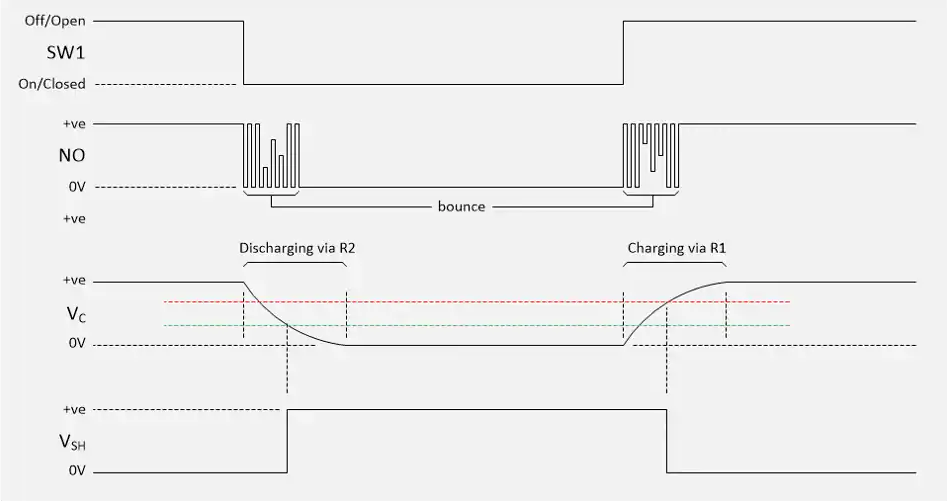
\includegraphics[width=\textwidth]{Assignment 5/2_hardware debouncing/graph.png}
            \caption{Hardware based Switch Debouncing (\href{https://www.digikey.com/en/articles/how-to-implement-hardware-debounce-for-switches-and-relays}{Source})}
            \label{fg14}
        \end{figure}

    \subsection{Conclusion}
        We discussed hardware based debouncing mechanism to reduce errors while taking input.
\newpage

\end{document}